\documentclass[a4paper]{article}
\usepackage[utf8]{inputenc}
\usepackage[russian,english]{babel}
\usepackage[T2A]{fontenc}
\usepackage[left=10mm, top=20mm, right=18mm, bottom=15mm, footskip=10mm]{geometry}
\usepackage{indentfirst}
\usepackage{amsmath,amssymb}
\usepackage[italicdiff]{physics}
\usepackage{graphicx}
\usepackage{multirow}
\usepackage{svg}
\graphicspath{{images/}}
\DeclareGraphicsExtensions{.pdf,.png,.jpg}
\usepackage{wrapfig}
\usepackage{caption}
\captionsetup[figure]{name=Рисунок}
\captionsetup[table]{name=Таблица}
\title{\underline{Получение и измерение вакуума}}
\author{Каспаров Николай, Б01-304}

\begin{document}

\maketitle
\begin{center}
\Large{\textbf{ }}
\end{center}

\subparagraph{Цель работы:}

1) Измерение объемов форвакуумной и высоковакуумной частей установки

2) Определение скорости откачки системы в стационарном режиме,
а также по ухудшению и улучшению вакуума

\subparagraph{В работе используются:}

Вакуумная установка с различными манометрами: масляным, термопарным, ионизационным.

\section{Установка}

Установка изготовлена из стекла и состоит из форвакуумного баллона
(ФБ), высоковакуумного диффузионного насоса (ВН), высоковакуумного
баллона (ВБ), масляного (М) и ионизационного (И) манометров, термопарных
манометров ($M_1$ и $M_2$), форвакуумного насоса (ФН) и соединительных
кранов ($K_1$, $K_2$,..., $K_6$) (Рис. 1). Кроме того, в состав установки входят:
вариатор (автотрансформатор с регулируемым выходным напряжением), или
реостат и амперметр для регулирования тока нагревателя диффузионного
насоса.


\begin{figure}[h]
    \centering
    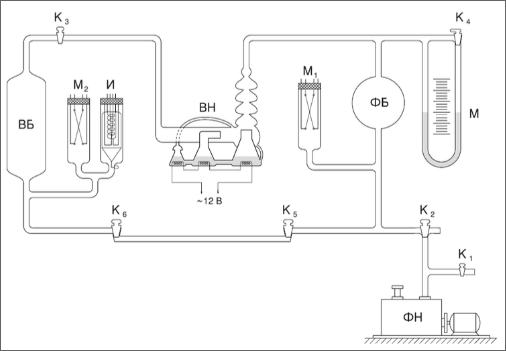
\includegraphics[scale=0.7]{ust.png}
    \caption{Схема установки}
\end{figure}

Кран $K_1$ используется для заполнения форвакуумного насоса и вакуумной
установки атмосферным воздухом. Во время работы установки он
должен быть закрыт. Трёхходовой кран $K_2$ служит для соединения форвакуумного
насоса с установкой или атмосферой. Кран $K_3$ отделяет высоковакуумную
часть установки от форвакуумной. Кран $K_4$ соединяет между
собой колена масляного манометра. Он должен быть открыт во все время
работы установки и закрывается лишь при измерении давления в форвакуумной
части. Краны $K_5$ и $K_6$ стоят по концам капилляра и соединяют
его с форвакуумной и высоковакуумной частями установки.

Устройство одной ступени масляного
диффузионного насоса схематически показано на Рис. 2
(в лабораторной установке
используется несколько откачивающих
ступеней). Масло, налитое в сосуд, подогревается электрической печкой.
Пары масла поднимаются по трубе и вырываются
из сопла. Струя паров увлекает молекулы
газа, которые поступают из откачиваемого
сосуда через трубку. Дальше смесь попадает
в вертикальную трубу. Здесь масло осаждается
на стенках трубы и маслосборников
и стекает вниз, а оставшийся газ откачивается форвакуумным насосом

\begin{figure}[h]
    \centering
    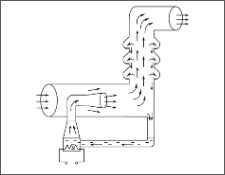
\includegraphics[scale=0.7]{ust2.png}
    \caption{Схема насоса}
\end{figure}

\subsection{Процесс откачки}

Производительность насоса определяется скоростью откачки $W$ (л/с):
$W$ — это объем газа, удаляемого из сосуда при данном давлении за единицу времени.
Скорость откачки форвакуумного насоса равна емкости воздухозаборной камеры,
умноженной на число оборотов в секунду.
Рассмотрим обычную схему откачки.
Разделим вакуумную систему на две части: «откачиваемый объем»
(в состав которого включим используемые для работы части установки)
и «насос», к которому, кроме самого насоса, отнесем трубопроводы и краны,
через которые производится откачка нашего объема.
Обозначим через $Q_d$ количество газа,
десорбирующегося с поверхности откачиваемого объема в единицу времени,
через $Q_i$ — количество газа, проникающего в единицу времени в этот объем извне
— через течи.
Будем считать, что насос обладает скоростью откачки $W$
и в то же время сам является источником газа; пусть $Q_n$ — поток газа,
поступающего из насоса назад в откачиваемую систему.
Будем измерять количество газа $Q_d$, $Q_i$ и $Q_n$ в единицах $PV$
(легко видеть, что это произведение с точностью до множителя $RT/ \mu$ равно массе газа).
Основное уравнение, описывающее процесс откачки, имеет вид

\begin{equation}
	-VdP=(PW-Q_d-Q_n-Q_i)dt
\end{equation}

Левая часть этого уравнения равна убыли газа в откачиваемом объеме $V$ , а правая определяет количество газа, уносимого насосом, и количество прибывающего вследствие перечисленных выше причин
за время $dt$. При достижении предельного вакуума (давление $P_{pr}$)

\begin{equation}
	\frac{dP}{dt}=0
\end{equation}

\begin{equation}
	W=\frac{\sum Q_i}{P_{pr}}
\end{equation}

Обычно $Q_i$ постоянно, a $Q_n$ и $Q_d$ слабо зависят от времени,
поэтому в наших условиях все эти члены можно считать постоянными.
Считая также постоянной скорость откачки $W$, получим:
\begin{equation}
    P - P_\text{пр} = P_0 - P_\text{пр} \exp \left( -\frac{W}{V} t \right),
\end{equation}
где $P_0$ - начальное давление. Оно велико по сравнению с $P_\text{пр}$, поэтому
можно записать:

\begin{equation}
    P = P_0 \exp \left( -\frac{W}{V} t \right)
\end{equation}

Постоянная откачки $\tau = \frac{V}{W}$ является мерой эффективности откачной системы.

\subsection{Течение газа через трубу}

Характер течения газа существенно зависит от соотношения между размерами системы
и длиной свободного пробега молекул.
При атмосферном давлении и даже при понижении давления
до форвакуумного длина свободного пробега меньше диаметра трубок
и течение откачиваемого газа определяется его вязкостью,
т.е. взаимодействием его молекул. При переходе к высокому вакууму картина меняется.
Столкновения молекул между собой начинают играть меньшую роль, чем соударения со стенками.
Течение газа в трубе напоминает в этих условиях диффузию газа
из области больших концентраций в области,
где концентрация ниже, причем роль длины свободного пробега играет ширина трубы.
Для количества газa, протекающего через трубу в условиях высокого вакуума или,
как говорят, в кнудсеновском режиме, справедлива формула:

\begin{equation}
\label{formula}
	\frac{d(PV)}{dt}=\frac{4}{3}r^3 \sqrt{\frac{2\pi RT}{\mu}} \frac{P_2-P_1}{L}.
\end{equation}
Применим эту формулу к случаю, когда труба соединяет установку с насосом.
Пренебрежем давлением $P_1$ у конца, обращенного к насосу.
Будем измерять количество газа, покидающего установку при давлении $P = P_2$.
Пропускная способность трубы:

\begin{equation}
	C_\text{тр}=(\frac{dV}{dt})_\text{тр}=\frac{4}{3}\frac{r^3}{L}\sqrt{\frac{2\pi RT}{\mu}}.
\end{equation}

Мы видим, что пропускная способность зависит от радиуса трубы в третьей степени
и обратно пропорциональна ее длине.
Поэтому в вакуумных установках следует поэтому применять широкие короткие трубы.

\section{Ход работы}

\subsection{Определение объёмов}

Объём, заключенный в кранах и капиллярах форвакуумной части при атмосферном давлении,
откроем на форвакуумную часть. Запишем показания масляного манометра:

\begin{equation}
    \Delta h_1 = (26.3 \pm 0.4) \ \text{см}
\end{equation}

Считая газ идеальным, можно записать:

\begin{equation}
    V_\text{фв} = \frac{p_0 V}{\rho g \Delta h_1} = (2160 \pm 40) \ \text{см}^3
\end{equation}

Откроем высоковакуумный баллон:

\begin{equation}
    \Delta h_2 = (16.9 \pm 0.4) \ \text{см}
\end{equation}

Аналогично получим:

\begin{equation}
    V_\text{общ} = (3360 \pm 80) \text{см}^3
\end{equation}
\begin{equation}
    V_\text{вв} = (1200 \pm 90) \text{см}^3
\end{equation}

\subsection{Измерение вакуума}

Откачав установку диффузионным насосом, с помощью ионизационного манометра 
измерим значение предельного давления:

\begin{equation}
    P_\text{пр} = (6.5 \pm 0.1) \cdot 10^{-5} \ \text{мм рт. ст.}
\end{equation}

Теперь найдём скорость откачки по ухудшению и улучшению вакуума,
для этого, открывая и закрывая кран 3, будем то подключать насос к
объёму, то отключать его. Результаты зафиксируем на графике

\begin{figure}[h]
    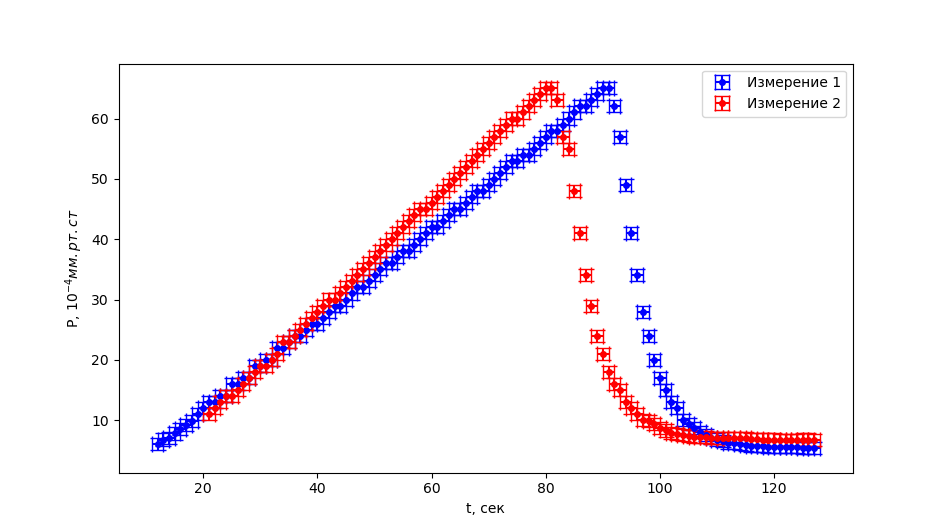
\includegraphics[scale=0.7]{Измерения1.png}
    \caption{Зависимость давления от времени}
\end{figure}

\begin{figure}[h]
    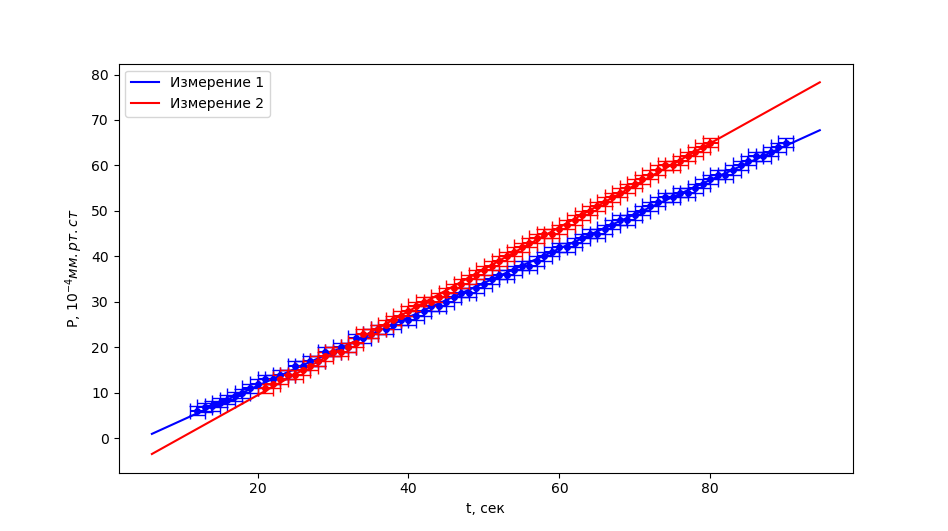
\includegraphics[scale=0.7]{Измерения2.png}
    \caption{Зависимость давления от времени при ухудшении вакуума}
\end{figure}

\begin{figure}[h]
    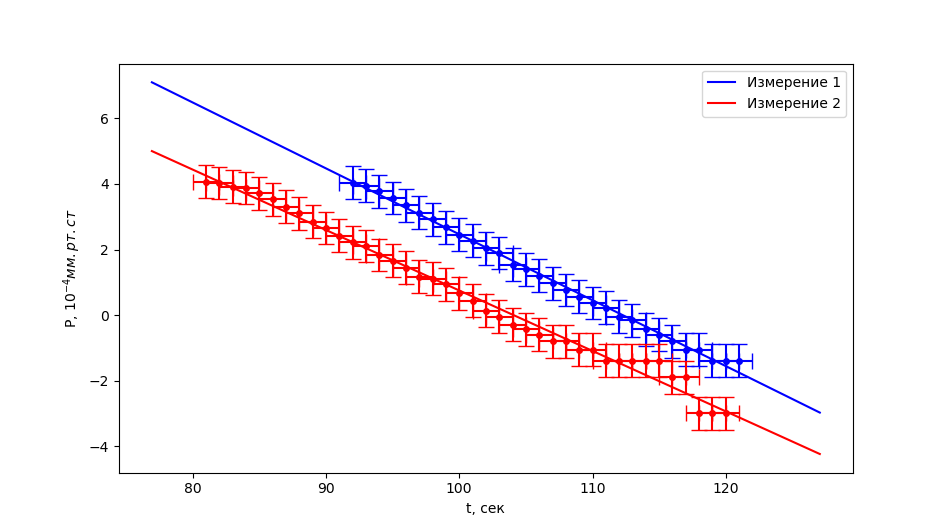
\includegraphics[scale=0.7]{Измерения3.png}
    \caption{Зависимость давления от времени при улучшении вакуума}
\end{figure}

Найдем коэффициенты наклона, используя МНК:

\begin{equation}
    k_\text{ухуд} = (0.841 \pm 0.002) \cdot 10^{-5} \frac{\text{мм рт. ст.}}{\text{с}}
\end{equation}

\begin{equation}
    k_\text{улуч} = (-0.196 \pm 0.002) \cdot 10^{-5} \frac{\ln(\text{мм рт. ст.})}{\text{с}}
\end{equation}

Тогда, используя $W = -kV$, тогда:

\begin{equation}
    W = (235 \pm 18) \frac{\text{см}^3}{c}
\end{equation}

Оценим величину потока газа $Q_\text{н}$.

\begin{equation}
(Q_\text{д} + Q_\text{и}) = \left( 1010\pm 80\right) \cdot 10^{-5} \frac{\text{мм. рт. ст.} \cdot \text{см}^3}{c}
\end{equation}

 Используя формулу $Q_\text{н} = P_\text{пр}W - (Q_\text{д} + Q_\text{и})$, получим, что: 
 
\begin{equation}
     Q_\text{н} = \left( 520\pm 140 \right) \cdot 10^{-5} \frac{\text{мм. рт. ст.} \cdot \text{см}^3}{c}
\end{equation}

\subsection{Пропускная способность трубы}

Оценим пропускную способность трубки:

\begin{equation}
    L = 10.8 \text{см}; \ d = 0.8 \text{мм}.
\end{equation}

\begin{equation}
    C_\text{тр} = 0.584 \ \frac{\text{см$^3$}}{c}.
\end{equation}

\subsection{Искусственная течи}

Введём в систему исскуственную течь и запишем значение установившегося при этом давления и давления в форвакуумной части установки: 

\begin{equation}
     P_\text{уст} = \left( 1.1\pm 0.1 \right) \cdot 10^{-4} \text{мм. рт. ст.}
\end{equation}
\begin{equation}
     P_\text{фв} = \left( 3.9\pm 0.1 \right) \cdot 10^{-3} \text{мм. рт. ст.}
\end{equation}

Поскольку

\begin{equation}
    P_\text{пр} W = Q_1, \quad P_\text{уст} W = Q_1 + \frac{d(PV)_\text{кап}}{dt}, 
\end{equation}

то 

\begin{equation}
    W = \frac{dV_\text{кап}}{dt}\frac{P_\text{фв}}{P_\text{уст}-P_\text{пр}} = \left( 51\pm 11 \right) \frac{\text{см}^3}{c}
\end{equation}

\section{Выводы}

К сожалению, результаты сошлись лишь порядком.
Это показывает несостоятельность второго метода измерения.

\begin{equation*}
    W_1 = (51 \pm 11) \frac{\text{см}^3}{c}
\end{equation*}
\begin{equation*}
    W_2 = (235 \pm 18) \frac{\text{см}^3}{c}
\end{equation*}



\end{document}
